\section{Multiplexingverfahren} \label{multiplex}
\begin{itemize}
  \item Zeitmultiplex - Time Division Multiple Access (TDMA), \textit{GSM, DECT, ISDN}
  \item Frequenzmultiplex - Frequency Division Multiple Access (FDMA), \textit{UKW-Radio}
  \item Codemultiplex - Code Division Multiple Access (CDMA), \textit{UMTS, GPS}
  \item Raummultiplex - Space Division Multiple Access (SDMA), \textit{Zellen der GSM-Basisstationen}
\end{itemize}

\skriptsubsection{FDM - Frequenzmultiplex (Frequency-Division Multiplexing)}{52}
Mit dieser Technik werden mehrer Modulierte Signale über ein Kanal gesendet. Die einzelnen
Trägerfrequenzen sind so ausgelegt, dass sich die Signale im gemeinsamen Kanal nicht überlagern und
kein Übersprechen stattfindet. Somit können die Nachrichtensignale unabhängig von den anderen
wieder demoduliert werden.
\begin{center}
    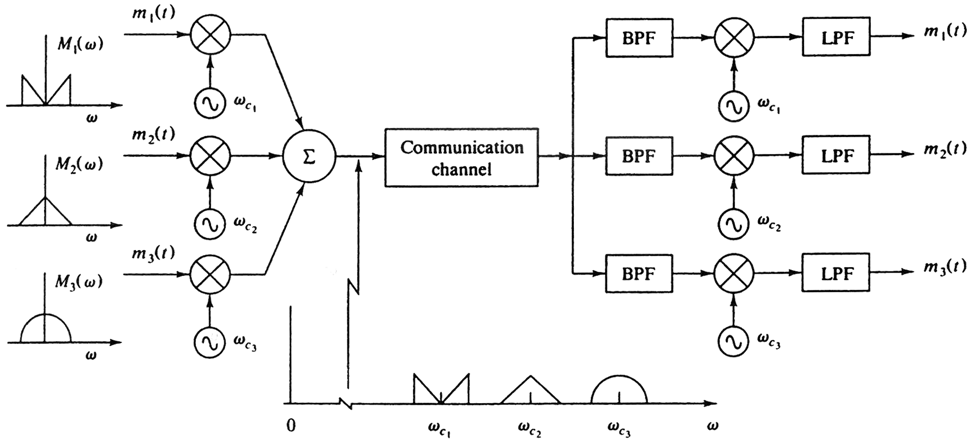
\includegraphics[width=14cm]{../NaT1/bilder/multiplex_fdm_blockdiagramm.png}
\end{center}

\skriptsubsection{TDM - Zeitmultiplex (Time-Division Multiplexing)}{100}
Bei TDM werden mehrere Nachrichtensignale über einen Kommunikationskanal gesendet, indem jedes
einzelne Signal jeweils nur zu bestimmten Zeitintervallen gesendet wird. Diese Umschaltung erfolgt
durch einen sogenannten Commutator. \\
Zeitmultiplex ist das wichtigste Mutiplexingverfahren für
Sprachübertragung inm Telekommunikationsnetz.
\begin{center}
    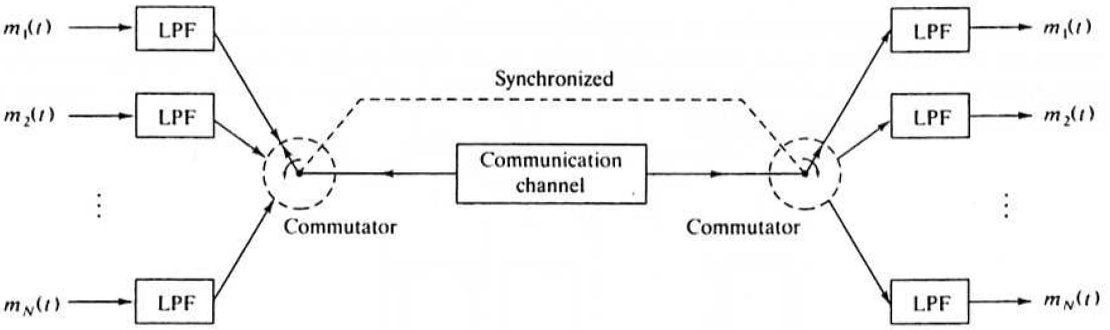
\includegraphics[width=14cm]{../NaT1/bilder/multiplex_tdm_blockdiagramm.png} \\
    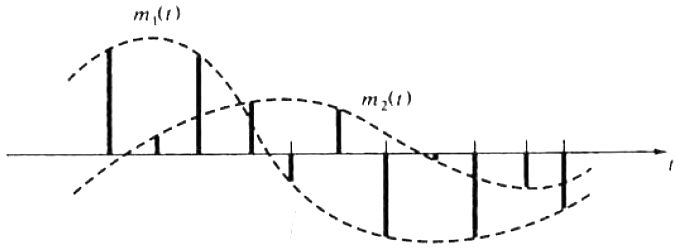
\includegraphics[height=3cm]{../NaT1/bilder/multiplex_tdm_zeitdiagramm.png}     
\end{center}